\chapter{Tutorial Visual Studio}
\label{cha:visualstudio}
\thispagestyle{empty}

We bespreken in deze bijlage het opzetten van een project in Visual Studio 2019. Visual Studio 2019 kan gedownload worden van de website van Microsoft. De precieze installatie van de software verschilt van computer tot computer, afhankelijk van de al eerder geïnstalleerde software, met name de \textsl{runtime libraries}.

Download Visual Studio Community via de link:

\hspace*{1em}\url{https://visualstudio.microsoft.com/vs/}

\textbf{Let op:} download de Community-editie. Zie figuur~\ref{fig:000Adownloadcommunity}.

\begin{figure}[H]
\centering
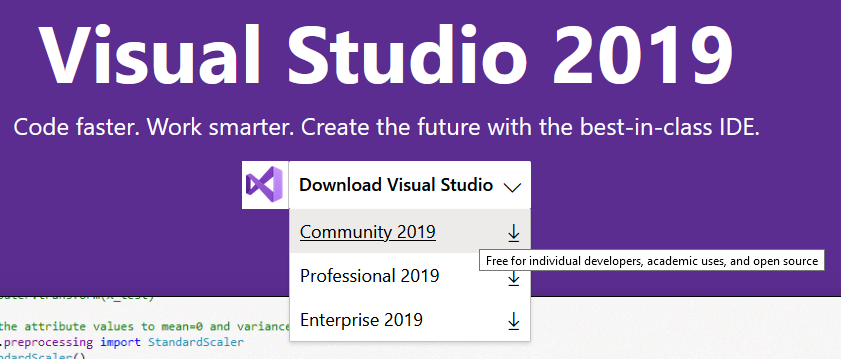
\includegraphics[scale=\figscaleAA]{images/000Adownloadcommunity}
\caption{Downloaden van Community-editie.}
\label{fig:000Adownloadcommunity}
\end{figure}

Er wordt nu een kleine installer gedownload. Start daarna de installer. Visual Studio is een groot programma, dus het kost nogal wat tijd om Visual Studio te installeren.

Visual Studio ondersteunt het ontwikkelen van applicatue met een veelzijdigheid aan mogelijkheden. Wij gebruiken de C/C++-compiler voor Desktop Development. Om te kunnen ontwikkelen moeten we een \textsl{workload} installeren. Selecteer de workload zoals te zien is in figuur~\ref{fig:000installworkload}. Selecteer de opties zoals is aangegeven aan de rechterkant van de figuur. Klik daarna op \texttt{Install while downloading}.

\begin{figure}[H]
\centering
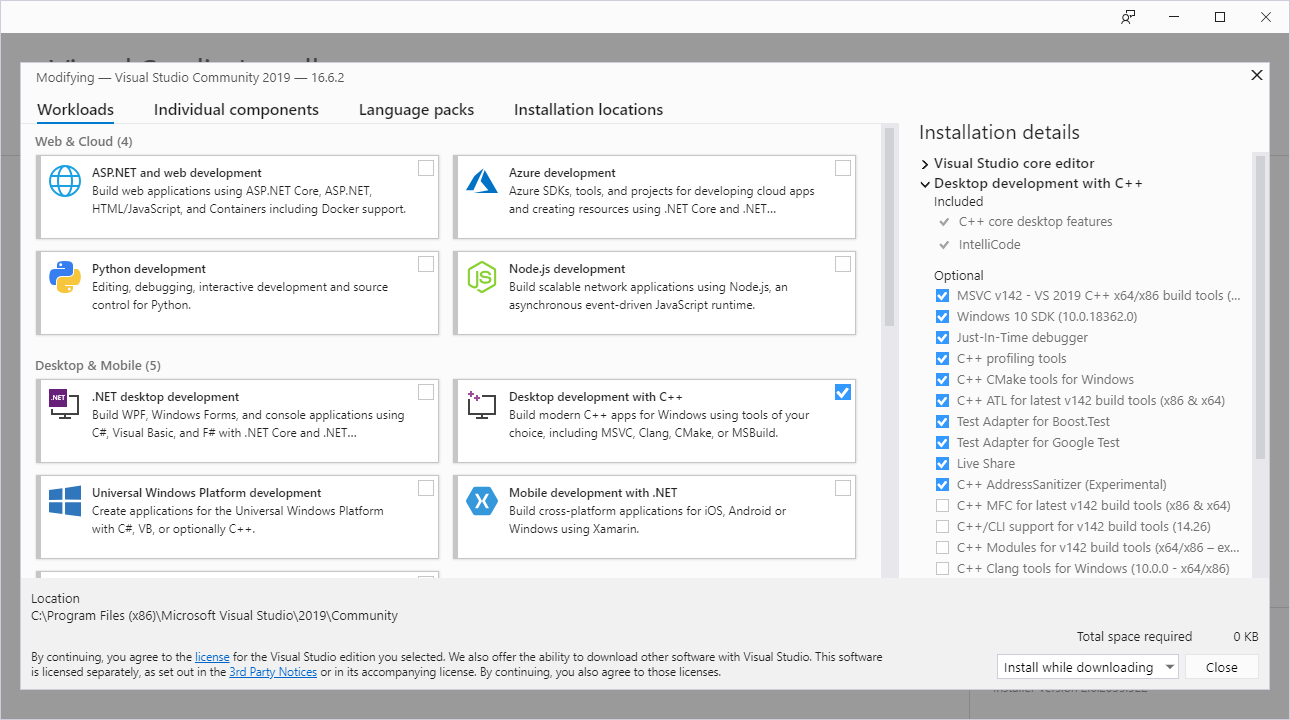
\includegraphics[scale=\figscaleAA]{images/000installworkload}
\caption{Selecteren van de C++-workload.}
\label{fig:000installworkload}
\end{figure}


Start Visual Studio door op het icoon te klikken. Visual Studio opent een beginscherm waarin een nieuw project kan worden aangemaakt. Dit is te zien in figuur~\ref{fig:001newproject}. Klik op het kader \texttt{Create a new project}.

\begin{figure}[H]
\centering
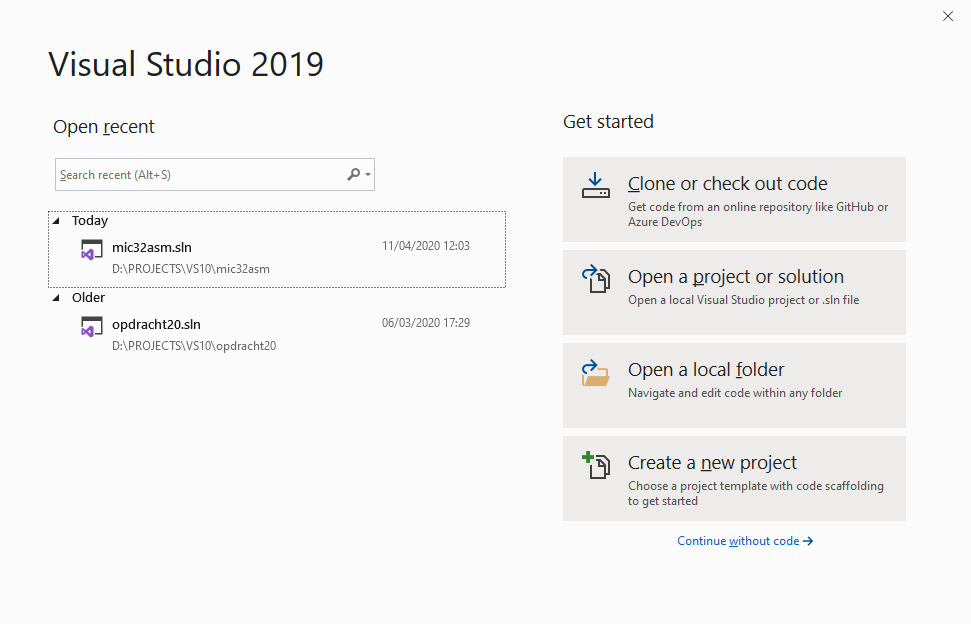
\includegraphics[scale=\figscaleH]{images/001newproject}
\caption{Aanmaken van een nieuw project.}
\label{fig:001newproject}
\end{figure}

Er wordt een nieuw scherm geopend, zie figuur~\ref{fig:002create}. Klik daarin op het kader \texttt{Empty Project}. \textbf{Klik niet op\texttt{ Console App}.}

\begin{figure}[H]
\centering
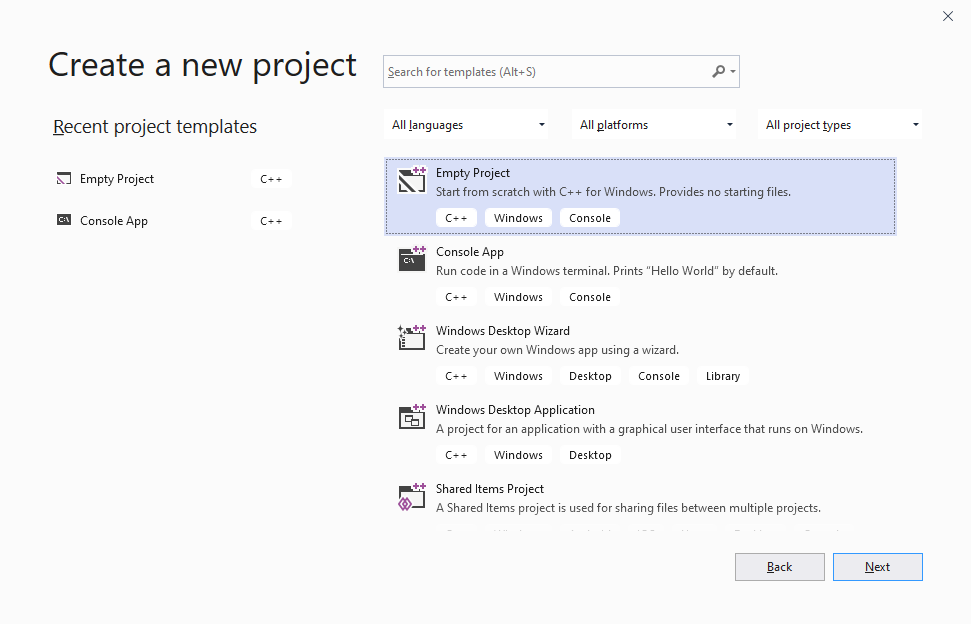
\includegraphics[scale=\figscaleH]{images/002create}
\caption{Aanmaken van een leeg project.}
\label{fig:002create}
\end{figure}

Daarna moeten wat gegevens worden ingevuld. Vul de projectnaam in en de map waarin het project terecht moet komen. Vink de checkbox onderaan aan en klik op de knop \texttt{Create}. Zie figuur~\ref{fig:003configure}.

\begin{figure}[H]
\centering
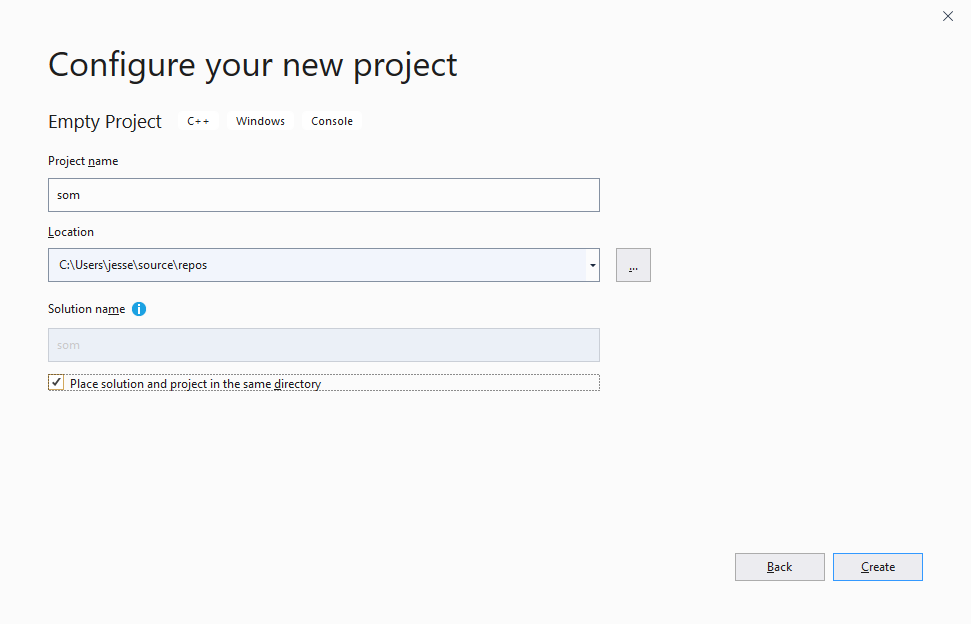
\includegraphics[scale=\figscaleH]{images/003configure}
\caption{Gegevens van het project invoeren.}
\label{fig:003configure}
\end{figure}

Visual Studio komt nu met het hoofdscherm waarin een aantal vensters (Engels: pane) te zien zijn. Er is nog geen C-bestand aangemaakt, dat moeten we zelf doen. In de \textsl{Solution Explorer} aan de rechterkant is een map \texttt{Source Files} te zien. Ga met de muis-pointer daar op staan en klik op de \textbf{rechter} muisknop.

Selecteer daarna de optie \texttt{Add} en daarna \texttt{New item..}. Zie figuur~\ref{fig:004addnewitem}.

\begin{figure}[H]
\centering
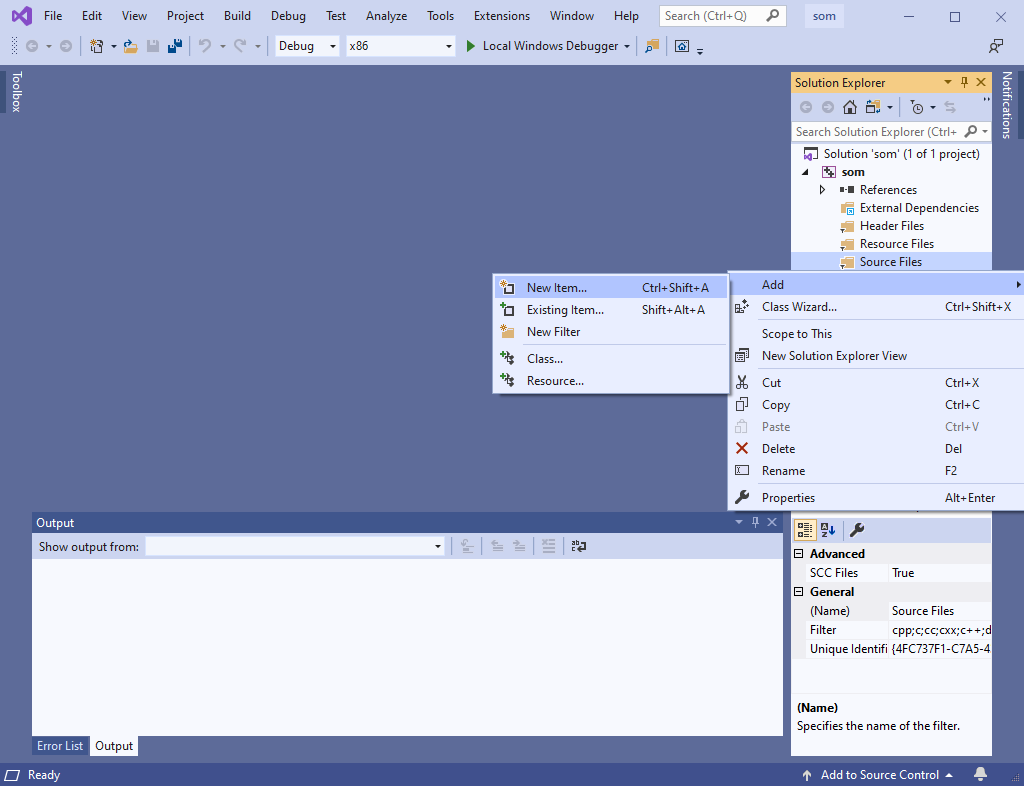
\includegraphics[scale=\figscaleH]{images/004addnewitem}
\caption{Een nieuw bestand aanmaken.}
\label{fig:004addnewitem}
\end{figure}

In het volgende scherm moet een bestandstype en een naam worden opgegeven. Klik op \texttt{C++ File (.cpp)}. Vul onderin bij  \texttt{Name} de naam van het bestand in \textbf{en zorg ervoor dat de naam eindigt met \texttt{.c}}, anders wordt een C++-bestand aangemaakt. Klik daarna op de knop \texttt{Add}. Zie figuur~\ref{fig:005enterfilename}.

Voer het programma in zoals te zien is in figuur~\ref{fig:006build}. Klik daarna op de knop \texttt{Local Windows Debugger}. Het programma wordt nu gecompileerd en als er geen fouten zijn gevonden, wordt het programma uitgevoerd. Herstel eventuele fouten die door de compiler gevonden worden en herstart de compilatie.

Het programma drukt de regel \texttt{De som van 3 en 7 is 10} af. Dit wordt gedaan in een zogenoemde \textsl{console}. Dit is te zien in figuur~\ref{fig:007output}.

De tutorial is hiermee ten einde.

\begin{figure}[H]
\centering
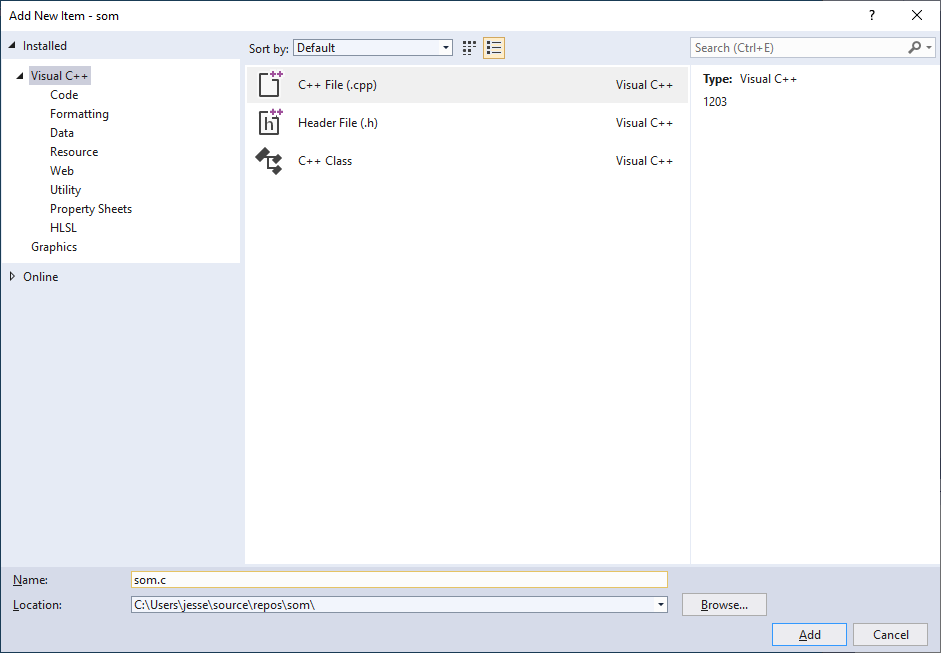
\includegraphics[scale=\figscaleH]{images/005enterfilename}
\caption{Gegevens van het C-bestand invullen.}
\label{fig:005enterfilename}
\end{figure}

\begin{figure}[H]
\centering
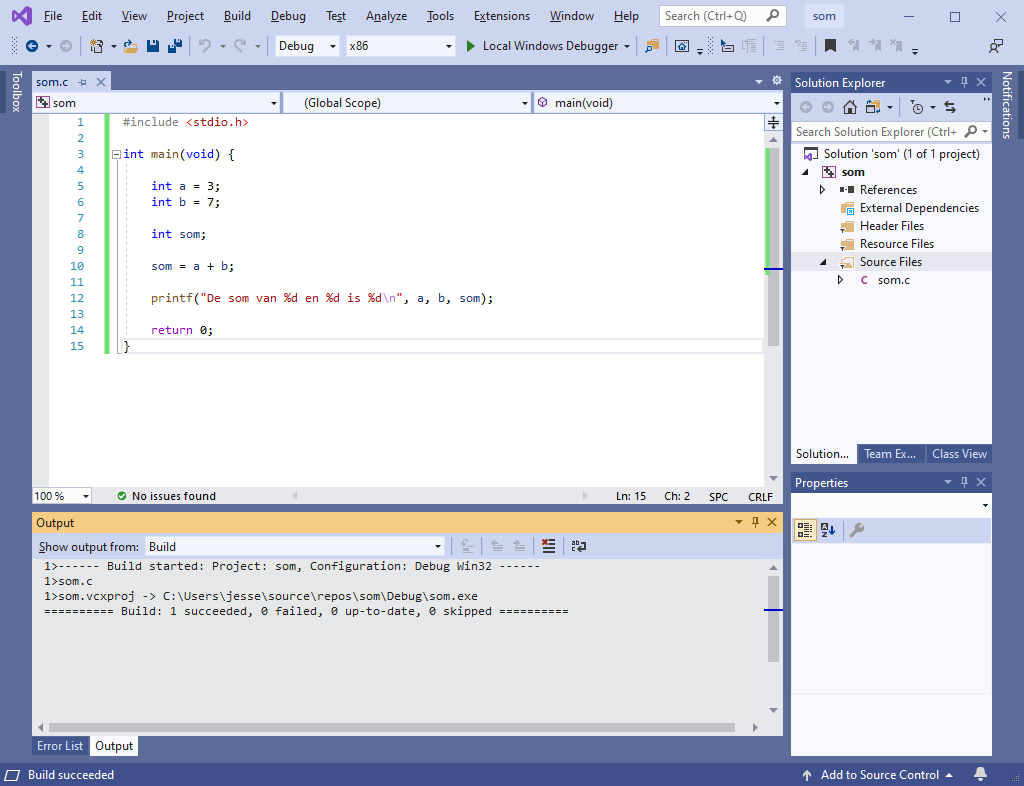
\includegraphics[scale=\figscaleH]{images/006build}
\caption{Compileren en starten van de executable.}
\label{fig:006build}
\end{figure}

\begin{figure}[H]
\centering
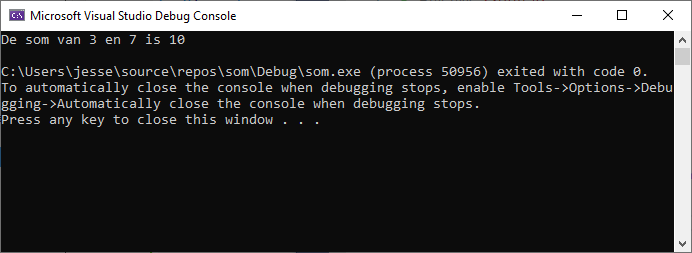
\includegraphics[scale=\figscaleH]{images/007output}
\caption{Uitvoer van het programma in een console.}
\label{fig:007output}
\end{figure}